% lec2.tex 
\divider 
\lecture{2}{08:06 AM Sun, Oct 05 2025}{} 
Let $a,b $ be a positive real number. set: 
\[
\mathcal{R} (t, x_0, a, b)  = 
\left\{ (t, x) \in  \Omega : \quad \left| t-t_0 \right| \leq a \text{ and } \| x-x_0 \| \leq b \right\}
\]
where $\| . \|  $ is an appropriate norm in $\RR ^{k}$. 
\begin{center}
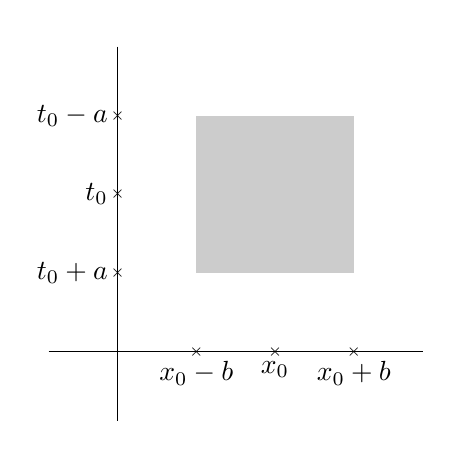
\begin{tikzpicture}
  \node[] (a) at (0, 0) {};
  \node[] (b) at (0, -5) {};

  \node[] (a2) at (-1, -4) {};
  \node[] (b2) at (4, -4) {};

  \draw[] (a) -- (b);
  \draw[] (a2) -- (b2);

  \node[anchor=north] at (1, -4) { $x_0-b$ };
  \node[anchor=north] at (1+1, -4) { $x_0$ };
  \node[anchor=north] at (1+2, -4) { $x_0+b$ };

  \node[] at (1, -4) { \tiny  $\times  $ }  ;
  \node[] at (1+1, -4) { \tiny $\times  $ } ;
  \node[] at (1+2, -4) { \tiny $\times  $ } ;
                                            
  \node[anchor=east] at (0, -1) { $t_0-a$ } ;
  \node[anchor=east] at (0, -2) { $t_0$ }   ;
  \node[anchor=east] at (0, -3) { $t_0+a$ } ;
                                            
  \node[] at (0, -1) {\tiny $\times$ }      ;
  \node[] at (0, -2) {\tiny $\times$ }      ;
  \node[] at (0, -3) {\tiny $\times$ }      ;

  \fill[opacity=0.5, gray!80] (1, -1) rectangle (3, -3);
\end{tikzpicture}
\end{center}
The rectangle $\mathcal{R}  $ is called a security system, its projection on $\RR  $ 
is called security interval and its projection on $\RR ^{k} $ which is 
$D = \left\{ \| x-x_0 \| \leq b\right\} $ is called security domain. \\
Suppose now that $f $ is continuous on $\mathcal{R}  $ and set: 
\[
M = \sup_{(t,x) \in \RR } \| f(t, x)  \| 
\]
and, 
\[
  \al = 
  \begin{cases}
    a \\
    \min \left( a, \frac{b}{M} \right)
  \end{cases}
  \begin{gathered}  
  \text{ if } M = 0 \\
  \text{ if } M \neq 0
  \end{gathered}
\]
% \begin{proposition}[]
% Let $\FF  $ be a solution to (I.V.P.1) defined on the interval $I = \left[ t_0 -\overset{\sim}{\al} , t_0 +\overset{\sim}{\al}\right]$ with 
% \[
%   \overset{\sim}{\al} 
% \leq  \al 
% \text{  
% \textcolor{red}{ $\leq a$}
% } 
% \]
% then: 
% \[
% \| \FF (t)  - x_0 \|  \leq  b  \quad \forall t \in  I
% \]
% In other words, $(t, \FF (t) ) \in \mathcal{R} (t_0, x_0, a, b) $ for all $t \in  I$.  
% \end{proposition}
% \begin{proof}
% Suppose that $\FF  $ is a solution to (I.V.P.1) with 
% $(t, \FF (t) ) \notin \mathcal{R}$, since $\FF  $ is continuous then there exists 
% $\bb \in (0, \overset{\sim}{\al} )  $ such that 
% $\| \FF (t) - x_0 \| < b$ for $ \left| t-t_0 \right|<  \bb $ and 
% \[
% \| \FF (t_0 \pm \bb) - x_0  \|  = b
% \]
% \end{proof}

\begin{proposition}[]
Let $\FF  $ be a solution to the IVP (IVP1) defined
on an interval $I_{\overline{\al}} = 
\left\{ t \in   \RR : \quad \left| t-t_0 \right|  < \overline{\al} \right\} = 
(t_0-\overline{\al}, t_0 + \overline{\al}) $, with 
$\overline{\al}\leq \al$, then $\| \FF (t) - x_0 \| < b \quad 
\forall  t \in   I_{\overline{\al}}$ 
\end{proposition}
\begin{proof}
Suppose that $\FF  $ is a solution to (IVP1), with 
$(t, \FF  (t) ) \notin  \mathcal{R} $ for 
$\left| t-t_0 \right|  < \overline{\al} $, since 
$\FF  $ is continuous, there exists $\bb \in   (0, \overline{\al})  $ such that $\| \FF (t) - x_0 \| < b $ for all
$\left| t-t_0 \right|  < \bb  $ and 
$\| \FF (t_0 \pm \bb ) - x_0  \|  = b$, hence we have: 
\[
\sup_{t \in  I_{\bb }, x \in   \overline{B}(x_0, b) } 
\| f(t, x)  \| \leq M
\]
Hence for all $\left| t-t_0 \right|  \leq \bb $, we have:
\begin{align*}
  \| \FF (t) - x_0  \|  &=
  \| \int_{t_0}^{t} f(s, \FF (s) ) ds \|  \\
  & \leq 
  M \left| t-t_0 \right|   \leq M \bb  \leq  b
  M\al \leq   b
\end{align*}
In particular for $t = t_0 \pm \bb  $.
\[
b = \| \FF (t_0 \pm \bb )  - x_0 \| < b
\]
contradiction.
\end{proof}
\begin{proposition}[]
If $\FF  $ is a solution to (IVP1) defined on $I = \left[ t_0 - \overset{\sim}{\al} , t_0  + \overset{\sim}{\al}  \right] $ 
with $\overset{\sim}{\al}  \leq  \al $, then: 
\[
\| \FF (t_1)  - \FF (t_2)  \|  \leq  M \left| t_1-t_2 \right| 
\quad \forall t_1, t_2 \in  I
\]
\end{proposition}
\noindent \textcolor{purple!90!blue}{
\ding{43} \textsc{Remark :}
} If $f $ is $\mathcal{C} ^{k} $ and $\FF  $ 
is a solution to (IVP1) then $\FF  $ is 
$\mathcal{C} ^{k+1} $.
\begin{proof}
From the integral form we have: 
\begin{align*}
  \| \FF (t_1)  - \FF (t_2)  \|  &= 
  \| \int_{t_1}^{t_2} f(s, \FF (s) ) ds  \|  
  \\
                                 &\leq  
  \int_{t_1}^{t_2}  
  \| f(s, \FF (s) )  \|  ds = M \left| t_1 - t_2 \right|
\end{align*}
\end{proof}
\section{Existence and Unicity}
\subsection{Local Existence and Uniqueness}
We use the following Banach contraction principle.
\begin{theorem}[]
Let $(E, d)  $  be a complete metric space and let $ T : E \longrightarrow E $ be a 
$k $-contraction (i.e. $k \in [0, 1) $) and for all 
$x,y \in  E $: 
\[
d(f(x) , f(y) )  \leq  k \cdot  d(x, y) 
\]
then in $I $, $T$ admits a unique fixed point $\overline{x}$ such that $T(\overline{x}) = \overline{x}  $. Moreover,
for any $x_0 \in  E $ the sequence 
$(x_n )_{n \in  \NN}  $ defined by $x_{n+1} = T(x_n )  $ converges to $\overline{x} $ and we have: 
\[
d(x_n , \overline{x})  \leq 
\frac{k^{n}}{1-k} \cdot d(x_1, x_0) 
\]
\end{theorem}
\begin{theorem}[Schauder]
Let $C $ be a nonempty closed convex set in a Banach space $E $ . 
Any compact mapping $ T : C \longrightarrow C $
(i.e. $T $ is continuous and $\overline{T(C) } $ is compact) admits a fixed point 
i.e. 
\[
\exists \overline{x}\in   C: \quad T(\overline{x})  = \overline{x}
\]
\end{theorem}
\begin{theorem}[]
Suppose that $f $ is $L- $ Lipschitzian with respect to $x $, i.e. 
\[
  \| f(t,x) - f(t, y)  \| \leq  L \| x-y \| 
\]
for all $x, y \in  \overline{B}(x_0, b) $ and for all $t \in  \left[ t_0 - \al, t_0 + \al \right] $. Then 
there exist $\dd  \in   (0, \al)  $ such that IVP (IVP1) has a unique solution $\FF  $ defined on 
$I_{\dd } = \left[ t_0 - \dd , t_0 + \dd  \right]$.
\end{theorem}
\begin{proof}
For any $\dd \in   (0, \al)  $ consider the mapping 
$ T_{\dd } : X \longrightarrow X$ defined by
\[
T_{\dd }x(t)  = x_0 + \int_{t_0}^{t} f(s, x(s) )  ds
\]
for all $x \in  X = \left\{  x  :  I_{\dd }\longrightarrow \RR ^{k}: \quad \text{ continuous}     \right\} $ endowed
by the sup-norm $\| . \| _{\infty } $ i.e.\\  $\| x \| _{\infty } = \sup_{t \in   I_{\dd }} \| x(t)  \| $. For
any $x,y \in   X $ and any $t \in   I_{\dd } $, we have 
\begin{align*}
  \| Tx(t) - Ty(t)   \|  &= \| \int_{t_0}^{t} f(s,x(s) )  ds\|  
  \\
                         & \leq \int_{\min (t, t_0) }^{\max (t, t_0) } 
                         \| f(s, x(s) ) - f(s, y(s) )  \| ds 
                         \\
                         & \leq L \int_{\min (t, t_0) }^{\max (t, t_0) } \| x(s)  - y(s)  \| ds
                         \\
                         & \leq L \| x-y \| _{\infty }\int_{ \min (t_0, t) }^{\max (t_0, t) } ds 
                         \\
                         & \leq L \left| t-t_0 \right|  \| x-y \| _{\infty }
                         \\
                         & \leq  L \dd  \| x-y \| _{\infty }
\end{align*}
so for $\dd  <  \frac{1}{L} $, $T_{\dd } $ is a contraction. Hence, for such a $\dd  $, 
$T_{\dd } $ has a unique fixed point $\ff \in  X $, i.e.  $ \ff  : I_{\dd } \longrightarrow \RR ^{k} $ 
with,
\[
\ff (t) = x_0 + \int_{t_0}^{t} f(s, \ff (s) ) ds,
\]
which is the unique solution to the IVP(IVP1).
\end{proof}
% \begin{theorem}[]
% Let $a, b $ be two positive real numbers, and set $\mathcal{R} = \mathcal{R} (t_0, x_0, a, b)  $, 
% let $ f : \mathcal{R}  \longrightarrow \mathcal{R} ^{k} $ be a continuous function such that 
% $\exists L \geq  0$ with: 
% \[
% \| f(t,x)  - f(t,y)  \|  \leq  L \| x-y \|  \quad \quad \forall (t, x) (t, y) \in \mathcal{R} 
% \]
% then there exists $\dd  \in  (0, \al)  $ such that 
% the I.V.P (IVP1) has a unique solution defined defined on: 
% \[
% I_{\dd } = 
% \left[ t_0 - \dd , t_0 + \dd  \right]
% \]
% hence, 
% \[
%   \al = \begin{cases}
%   a \\
%   \min  \left( a, \frac{b}{M} \right) \\
%   \end{cases}
%   \begin{gathered}  
%   \text{ if } M = 0 \\ 
%   \text{ if } \sup_{(t, x) \in  \mathcal{R} }  
%   \| f(t, x)  \| > a \\
%   \end{gathered}
% \]
% \end{theorem}
% \begin{proof}
% Let $X = C \left[ t_0 - \dd , t_0 + \dd  \right] $ , endowed 
% with the sup-norm $\| . \| _{ 0 } $, i.e.: 
% \[
% \| x \| _{0} = 
% \sup_{t \in \left[ t_0 - \dd , t_0 + \dd  \right]} 
% \left| x(t)  \right|
% \]
% Consider the mapping:
% \[
% \begin{array}{cccc}
%       T : &  X  & \longrightarrow & X \\
% 
%            &  x(t)   & \longmapsto     & T x(t) = x_0+ \int_{t_0}^{t} 
%            f(s, x(s) ) ds\\ 
% \end{array}
% \]
% Let 
% \[
% S = \left\{ x \in  X: \| x-x_0 \| \leq b \right\}
% \]
% Its clear that $\FF  $ is a fixed point of 
% $I $. then $\FF  $ is a solution to IVP (IVP1). \\
% \underline{\emph{1$^{st}$ step:}} to be continued
% \end{proof}
% end of file
